\documentclass[11pt,a4paper]{report}

\usepackage{datetime}
\usepackage{graphicx}
\usepackage{enumitem}
\usepackage{amsmath}

\title{Theoretical Answer}
\newdate{date}{28}{06}{2020}
\date{\displaydate{date}}
\author{Nguyen Ngoc Lam}


\begin{document}
  	\pagenumbering{arabic}
  	\tableofcontents
  	\newpage
	
	\chapter{Chapter 1: Overview of Distributed Systems}
	\newpage
  	\section{Role of Middleware in A Distributed System}
  	Middleware aims at improving the single-system view that a distributed system should have. In other word, to enhance the distribution transparency that is missing in network operating systems.
  	
  	\section{Distribution Transparency and Example}
  	Distribution transparency is the phenomenon by which distribution aspects
in a system are hidden from users and applications. \\
Examples include access transparency, location transparency, migration transparency, relocation transparency, concurrency transparency and failure transparency.

 	\section{Reason for Why It Is Hard to Hide the Occurrence and Recovery From Failures in a Distributed System}
  	It is generally impossible to detect whether a server is actually down, or
that it is simply slow in responding.

  	\section{Why It Is Not always a Good Idea to Aim at Implementing the Highest Degree of Transparency Possible}
  	There is a trade-off between high degree of transparency and users accepted performance. If you try to aim to implement the highest degree of transparency, it could lead to slower-than-accepted performance.
  	
	\section{An Open Distributed System and Benefits}
	An open distributed system offers services according to clearly defined
rules. \\
An open system is not only capable of easily interoperating with other open systems but also allows applications to be easily ported between different implementations of the same system.

	\section{A Scalable System}
	A system is scalable when it can grow in one or more dimensions, with respect to either its number of components, geographical size or number and size of administrative domains, without an unacceptable loss of performance.
	
	\section{Different Techniques of Scalability}
	Scaling can be achieved through distribution, replication, and caching.
	
	\chapter{Chapter 2: Architectures}
	\newpage
  	
  	\section{Problem of Physical Distance}
  		From what I gathered, the physical distance only has a significant affect on latency if you are to implement a system that capture a live data and than process it in almost real time for scientific purpose. If you built that kind of system (strongly depend on time), a simple solution would be to put the processing station near the source of information and then transmit a processed file.\\
  		Some of the common strategies to deal with latency are:
  		\begin{itemize}
  			\item caching data on the client - i.e. avoiding to make request again if possible
    		\item combining several smaller requests into bigger ones
    		\item compressing the request
    		\item reusing the same connection for many requests
    		\item using different protocols (i.e. a lot of games use UDP to avoid latency at the cost of making other things much more complex)
    		\item caching data on the server
    		\item redesigning the way to make requests (pre-loading data, pre-allocating resources, creating parallel requests)
    		\item using content delivery networks (CDN) for static data
    		\item running a code through a profiler and redesigning it to eliminate bottlenecks
    		\item minimizing critical sections of code
    		\item designing the service as stateless so that it can be deployed on many servers in parallel
    		\item correctly sizing, designing and maintaining the system (OS, database, virtualization, load balancers, DNS caches, etc.)
    		\item correctly sizing, designing and maintaining the network (having enough bandwidth, using fast routers, traffic prioritization, resource reservation)
  		\end{itemize}
  	\section{Three-tiered Client-server Architecture}
  		A three-tiered client-server architecture consists of three logical layers, where each layer is implemented at a separate machine, in principle. The highest layer consists of a client user interface, the middle layer contains the actual application, and the lowest layer implements the data that are being used.
  	\section{Differences Between a Vertical Distribution and a Horizontal Distribution}
  		\begin{itemize}
  			\item Vertical distribution refers to the distribution of the different layers in a multitiered architectures across multiple machines. In principle, each layer is implemented on a different machine.
			\item Horizontal distribution deals with the distribution of a single layer across multiple machines, such as distributing a single database.
  		\end{itemize}
  	\section{Disadvantage of Topology of the Overlay}
  	The main problem here is dealing with logical paths. In practice, two nodes A and B which are neighbours in the overlay network may be physically placed far apart. As a result, the logically short path between A and B in this instance required routing a message along a very long path in the underlying physical network.
  	\section{Main Problems with Sequential Organization when Taking a Look at the Request-reply Performance at Process $P_1$ (The Last One)}
  		\begin{itemize}
  			\item Performance can be expected to be bad for large n since the problem is that each communication between two successive layers is, in principle, between two different machines.
  			\item The performance between $P_1$ and $P_2$
may also be determined by $n-2$ request-reply interactions between the other
layers.
			\item Another problem is that if one machine in the chain performs badly or is even temporarily unreachable, then this will immediately degrade the performance at the highest level.
  		\end{itemize}
	\section{Goodness of Routing Policy that Forward messages to the Closest Node Toward the Destination}
		According to the pictures of the question sheet, consider forwarding message from node $(0.2;0.3)$ (called $A$) to node $(0.9, 0.6)$ (called $B$). There are 2 routes:
		\newpage
		\begin{figure}[h!]
  			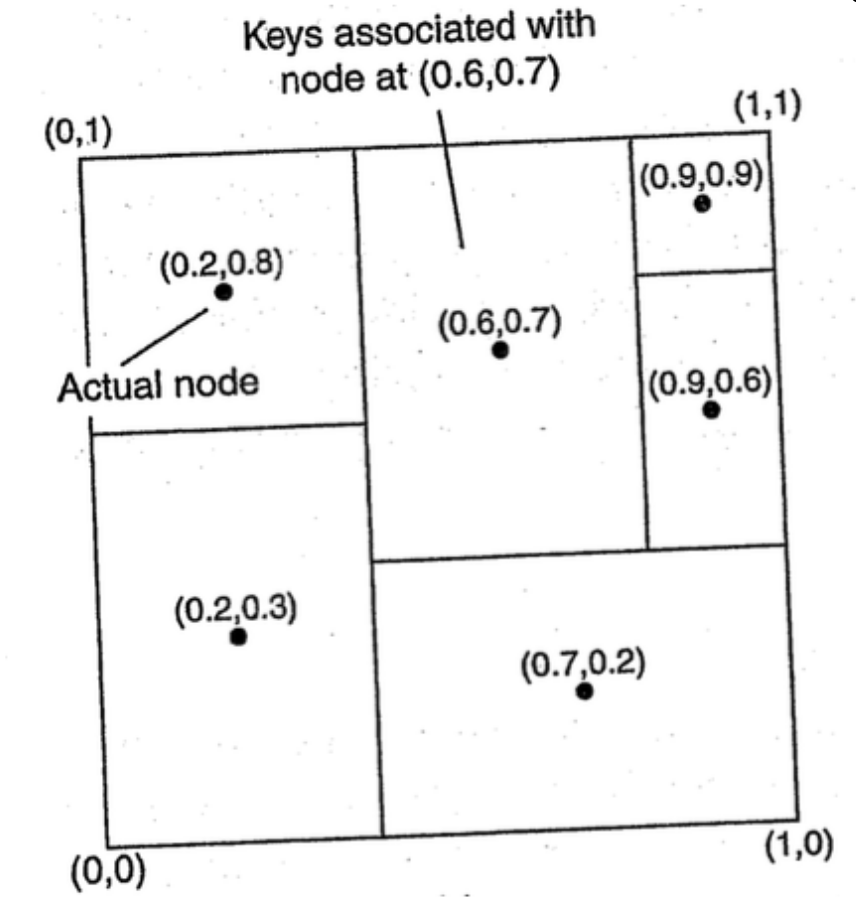
\includegraphics[width=\linewidth]{can-map.png}
  			\caption{CAN network}
  			\label{fig:CAN}
		\end{figure}
		\begin{enumerate}
			\item $A$, through $(0.6;0.7)$ (called $C$), to $B$:
				\[AC = \frac{2\sqrt{2}}{5} \approx 0.566\]
				\[CB = \frac{\sqrt{10}}{10} \approx 0.316\]
				\[TotalDistance = \frac{\sqrt{10} + 4\sqrt{2}}{10} \approx 0.882\]
			\item $A$, through $(0.7;0.2)$ (called $D$), to $B$:
				\[AD = \frac{\sqrt{26}}{10} \approx 0.510\]
				\[DB = \frac{\sqrt{5}}{5} \approx 0.447\]
				\[TotalDistance = \frac{\sqrt{26} + 2\sqrt{5}}{10} \approx 0.957\]
		\end{enumerate}		
		Because our policy is to forward a message to the closest
node toward the destination, which in this case D, we will actually go a little longer than if we take route 1. In conclusion, this policy is a reasonable one, but it is not always the best one.
	\section{Benefits of Microservices Architecture Compared To Monolithic Architecture}
		\begin{itemize}
			\item Microservices architecture makes systems and applications much faster to develop, and much easier to understand and maintain since it tackles the problem of complexity by decomposing application into a set of manageable services.
			\item Microservices architecture enables several teams to works on a projects, each can focus on one service or serveral closely-related services thus allowed services to be developed independently. 
			\item  Microservices architecture reduces barrier of adopting new technologies since the developers are free to choose whatever technologies make sense for their service and not bounded to the choices made at the start of the project.
			\item Microservice architecture makes continuous deployment possible for complex applications because it enables each microservice to be deployed independently.
			\item Microservice architecture enables each service to be scaled independently.
		\end{itemize}
	\section{Design an E-commerce System Using Microservices Architecture}
	Services in the system:
	\begin{itemize}
		\item HTTP apache: Get the HTTP request and forward it to the right service
		\item Customer: Handling customer data like: name, address, age, gender , preferences et cetera
		\item Order: Handling order information: who buying, from whom, what sort of item/items, how many item and for how much
		\item Catalogue: Handling item information: of what category, how many variants (colour, size, shape, version), contain what items (for bundle), how many items left, unit price, rating
		\item Vendor: Handling vendor information: name, address, vendor rating, what items are they selling, number of items sold in a time period (for customer to know if they have been receiving lots of requests)
	\end{itemize}
	\begin{figure}[h!]
  			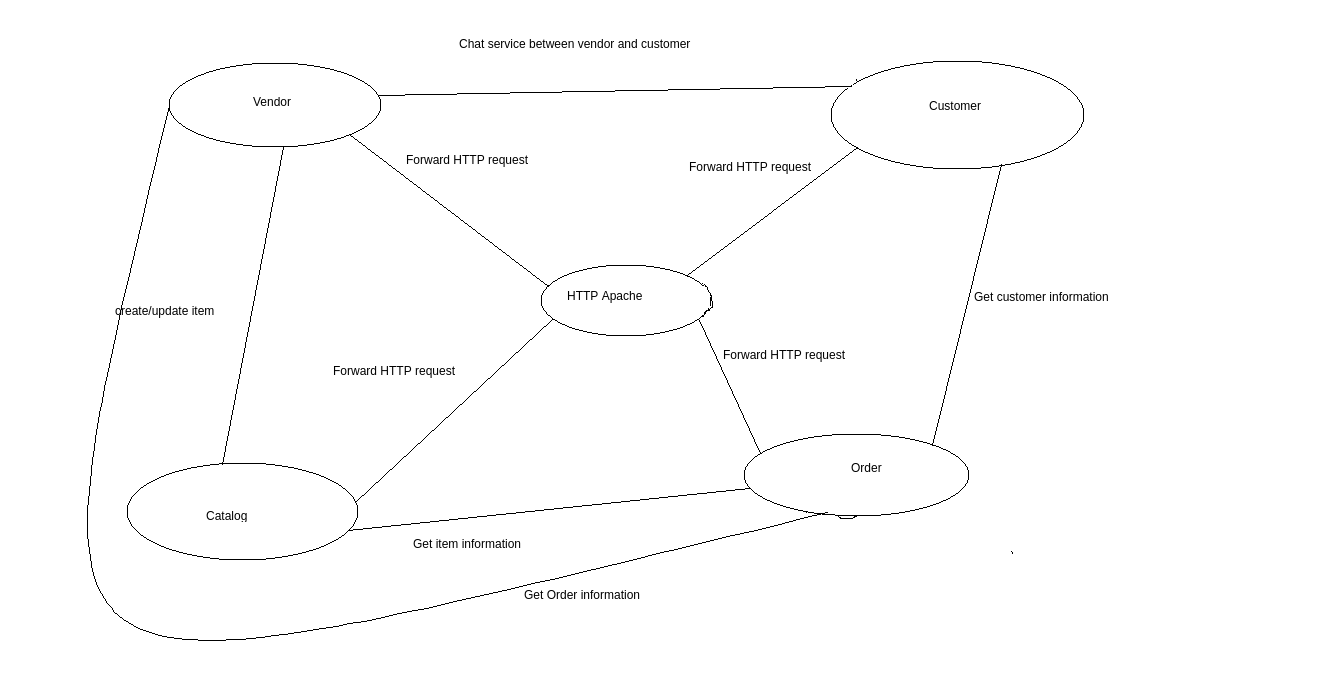
\includegraphics[width=\linewidth]{e-comm.png}
  			\caption{Figure to illustrate how the system interact}
  			\label{fig:ecomm}
		\end{figure}
		
	\chapter{Chapter 3: Processes and Threads}
	\newpage
  	
  	\section{Compare Process with Thread}
  	\begin{tabular}{|c|c|}
  	\hline 
  	\textbf{Process} & \textbf{Thread} \\ 
  	\hline 
  	System calls needed. & No system calls involved. \\ 
  	\hline 
  	Context switching required. & No context switching required. \\ 
  	\hline 
  	Different process have different  & Sharing same copy of \\ copies of code and data. & code and data can be possible \\ & among different threads. \\
  	\hline 
  	Operating system treats &  All user level threads treated as \\different process differently. & single task for operating system. \\ 
  	\hline 
  	If a process got blocked,  & If a user level thread got blocked, \\ remaining process continue & all other threads get blocked since \\their work & they are single task to OS. \\ 
  	\hline 
  	Processes are independent. & Threads exist as subsets of  \\ &a process. They are dependent. \\ 
  	\hline 
  	Process run in separate  & Threads run in shared memory space.\\ memory space. & memory space. And use memory  \\ & of process which it belong to.\\ 
  	\hline 
  	Processes have their own & Threads share Code section, \\ program counter (PC), register set& data section, address space \\  and stack space. & with other threads.\\
  	\hline 
  	 Communication between processes  & Communication between processes \\ requires some time. &requires less time than processes. \\ 
  	\hline 
  	Processes don’t share the memory & Threads share the memory with\\with any other process. & other threads of the same process \\ 
  	\hline 
  	Process have overhead. & Threads have no overhead. \\ 
  	\hline 
  	\end{tabular}
  	
  	\section{Limit the Number of Threads in a Server Process}
  	Yes, for two reasons. 
  	\begin{itemize}
  		\item First, threads require memory for setting up their own private stack. Consequently, having many threads may consume too much memory for the server to work properly.
  		\item Secondly, to an operating system, independent threads tend to operate in a chaotic manner. In a virtual memory system it may be difficult to build a relatively stable working set, resulting in many page faults and thus I/O. Having many threads may thus lead to a performance degradation resulting from page thrashing. \textbf{(more important)}.
  	\end{itemize}
  	
  	\section{Lightweight Process}
  		\subsection{As a Solution of Combining Advantages of Deploying Thread Package in User and Kernel Space}
  		\begin{itemize}
  			\item Responsiveness
  			\item Resource Sharing
  			\item Economy
  			\item Utilization of Multiprocessor Architectures
  		\end{itemize}
  		\subsection{A Single Lightweight Process per Process Is Not A Good Idea}
  		Such an association effectively reduces to having only kernel-level
threads, implying that much of the performance gain of having threads in the
first place, is lost.

	\section{Advantages of Multi-threaded Server Compared to Single-threaded Server}
	\begin{itemize}
		\item All the threads of a process share its resources thus making it more economical.
		\item Program responsiveness allows a program to run even if part of it is blocked using multithreading.
		\item Increase concurrency of the system since each thread can run on different processor.
	\end{itemize}
	\section{Advantages and Disadvantages of Each of Three Models of Multi-threaded Server}
		\subsection{Thread-per-request}
			\subsubsection{Advantages}
			\begin{itemize}
				\item The main advantage of thread-per-request is that it is  straightforward to implement.
				\item This architecture is particularly useful to handle long-duration requests, such as database queries, from multiple clients.
			\end{itemize}
			\subsubsection{Disadvantages}
			\begin{itemize}
				\item Thread-per-request can consume a large number of OS resources if many clients make requests simultaneously.
				\item It is inefficient for short-duration requests because it incurs excessive thread creation overhead.  
				\item It architectures are not suitable for real-time applications since the overhead of spawn a thread for each request can be non-deterministic.
			\end{itemize}
		\subsection{Thread-per-connection}
			\subsubsection{Advantages}
			\begin{itemize}
				\item Thread-per-connection is straightforward to implement.
				\item It is well suited to perform long-duration conversations  with multiple clients.
			\end{itemize}
			\subsubsection{Disadvantages}
			\begin{itemize}
				\item Thread-per-connection does not support load balancing effectively.
				\item For clients that make only a single request to each server, thread-per-connection is equivalent to the thread-per-request architecture.
			\end{itemize}
		\subsection{Thread-per-object}
			\subsubsection{Advantages}
			\begin{itemize}
				\item Thread-per-object is useful to minimize the amount of rework required to multi-thread existing single-threaded servants given that all methods in a servant only access servant-specific state there is no need for explicit synchronization operations.				
			\end{itemize}
			\subsubsection{Disadvantages}
			\begin{itemize}
				\item Thread-per-object does not support load balancing effectively since it serializes request processing in each servant. 
				\item Therefore, if one servant receives considerably more requests than others it can become a performance bottleneck. 
				\item It is prone to deadlock on nested callbacks.				
			\end{itemize}
	
	\section{Server Following Finite State Machine}
		\subsection{Example}
		Node.js is an example of a server following Finite state machine
		\subsection{Reason for its High Scalability}
		While single threaded, Node.js is asynchronous so a lot of requests can run on the single thread very quickly.
	\section{The Need of Multi-threaded for Client in Distributed Systems}
	In a single-process, single-threaded environment all requests to, e.g., the I/O interface blocks any further progress in the process. Any combination of a multi-process or multi-threaded implementation of the library makes provision for the user of the client application to request several independent documents at the same time without getting blocked by slow I/O operations.\\
	\textbf{Example:} As a World-Wide Web client is expected to use much of the execution time doing I/O operation such as "connect" and "read", a high degree of optimization can be obtained if multiple threads can run at the same time.
	\section{The Need of Virtualization Technology}
	\begin{itemize}
		\item Reduce Downtime
		\item Save Money and Time
		\item Better Recovery When Critical Error Happened
	\end{itemize}
	\section{Reason Why X-Window system Suitable for Thin Client Architecture}
	\begin{itemize}
		\item X is an architecture-independent system for remote graphical user interfaces and input device capabilities.
		\item Each person using a networked terminal has the ability to interact with the display with any type of user input device.
		\item X provides the basic framework, or primitives, for building such GUI environments: drawing and moving windows on the display and interacting with a mouse, keyboard or touchscreen
		\item A Thin Client Architecture is system where the clients (the application that runs on a personal computer or workstation and relies on a server to perform some operations) does very little. They basically just act as terminal for the server.
		\item This architecture allows disk-less client and make data storage more centralized.
		\item Since X is a windowing system, meaning it manages separated screens, it is suitable for thin client architecture as X-Window system does not require much client-side 
	\end{itemize}
	\section{Compare the Daemon Server and Superserver}
		\subsection{Daemon}
		In multitasking computer operating systems, a daemon is a computer program that runs as a background process, rather than being under the direct control of an interactive user. It means that daemon will always run as long as the system is still up.\\
		When finding a server, since the daemon is always running, you just need to call that particular daemon. However, many daemon may limit the performance of the hardware system. In addition, when needed, application may have to 'remember' the exact daemon for the job.
		\subsection{Superserver}
		Superserver is a kind of daemon that called necessary servers when they are needed.\\
		When finding a server, client will call directly to superserver. The downside of this is that the response time might be high.
		
		\chapter{Chapter 4: Communication}
		\newpage
  	
  	\section{Why in many layered protocols, each layer has its own header}
  	\begin{itemize}
  		\item Each layer must be independent of the other ones.
  		\item The data passed from the upper layer down to the lower layer contains both header and data, but the lower layer cannot tell which is which.
  		\item Having a single big header that all the layers could read
and write would make changes in the protocol of one layer visible to other layers, thus making the whole protocols unsafe.
  	\end{itemize}
  	
  	\section{Socket representation; Socket connection representation? Why do we need 4 values to represent a socket connection?}
  	A Socket is represented by:
  	\begin{itemize}
  		\item address
  		\item port
  	\end{itemize}
  	A Socket Connection is represented by;
  	\begin{itemize}
  		\item local-address
  		\item local-port
  		\item foreign-address
  		\item foreign-port
  	\end{itemize}
  	Why do we need 4 values to represented a socket connection:
  	\begin{itemize}
  		\item Each socket has 2 fields: address and port
  		\item A Socket Connection is defined by 2 sockets: local and foreign
  		\item To represent a Connection, we need to represent that 2 sockets
  	\end{itemize}
  	
  	\section{Three characteristics of TCP protocol}
  	\begin{itemize}
  		\item \textbf{\emph{Connection-Oriented}}: TCP requires that devices first establish a connection with each other before they send data. The connection creates the equivalent of a circuit between the units, and is analogous to a telephone call. A process of negotiation occurs to establish the connection, ensuring that both devices agree on how data is to be exchanged.
  		\item \textbf{\emph{Reliable}}: Communication using TCP is said to be \emph{reliable} because TCP keeps track of data that has been sent and received to ensure it all gets to its destination. As we saw in the previous topic, TCP can't really “guarantee” that data will always be received. However, it \emph{can} guarantee that all data sent will be checked for reception, and checked for data integrity, and then retransmitted when needed. So, while IP uses “best effort” transmissions, you could say TCP \emph{tries harder}, as the old rent-a-car commercial goes.
  		\item \textbf{\emph{Synchronous}}: All transmissions in TCP are \emph{acknowledged} (at the TCP layer—TCP cannot guarantee that all such transmissions are received by the remote application). The recipient must tell the sender \emph{“yes, I got that”} for each piece of data transferred, which is different from typical messaging protocols where the sender never knows what happened to its transmission
  	\end{itemize}
  	On UDP, they are:
  	\begin{itemize}
  		\item Connection-less
  		\item Unreliable: since it did not provide acknowledgement messages, it can not check whether the messages are received
  		\item Does not provide acknowledgement messages
  	\end{itemize}
  	
  	\section{Two main issues of RPC}
  	Issues:
  	\begin{itemize}
  		\item \textbf{\emph{Marshalling}}:Parameters must be marshalled into a standard representation.
  		\item \textbf{\emph{Binding}}: How does the client know who to call, and where the service resides?
  	\end{itemize}
  	
  	\section{Consider a procedure incr with two integer parameters. The procedure adds ONE to each parameter. Now suppose that it is called with the same variable twice, for example, as incr(i, i). If i is initially 0, what value will it have afterward if call-by-reference is used? How about if copy/restore is used?}
  	If call by reference is used, a pointer to $ i $ is passed to $incr$. It will be incremented two times, so the final result will be two. However, with copy/restore,$ i $ will be passed by value twice, each value initially 0. Both will be incremented, so both will now be 1. Now both will be copied back, with the second copy overwriting the first one. The final value will be 1, not 2.
  	
  	\section{Explain why transient synchronous communication has inherent scalability problems, and how these could be solved}
  	Problems:
  	\begin{itemize}
  		\item Scalability is the ability for a distributed application to expand without affecting any of the application algorithms.
  		\item The transient synchronous communication would have issues pertaining to geographical scalability. If the client and the server are placed in two far-away geographical locations it would take a considerable amount of time for the client to send a request and receive a reply.
  		\item Because the client remains idle until it receives the reply there is a considerable waste of time, since the client can only resume after receiving the reply. If the system is always in idle mode all of the time as it is synchronous there would not be any room for scalability.
  		\item This issue is a performance issue which creates unnecessary network latency.
  		\item There is set back when it comes to expanding of the system because it is transient system there is no storage. If there was to be a malfunction or failure of one component the whole system would be down. This is because the system is not persistent.
  	\end{itemize}
	Solutions:
	\begin{itemize}
		\item We can use network optimization tools. These tools help to minimize the amount traffic being built up on the network.
		\item Another solution would be to change to a new upgraded network connection. A faster network connection is key factor to reduce the time taken to receive a reply for request sent to the server from the client.
	\end{itemize}

	\section{Can we apply the persistent asynchronous communication to RPC? Explain it}
	Yes, but only on a hop-to-hop basis in which a process managing a queue
passes a message to a next queue manager by means of an RPC.\\
	Effectively, the service offered by a queue manager to another is the storage of a message. The calling queue manager is offered a proxy implementation of the interface to the remote queue, possibly receiving a status indicating the success or failure of each operation. In this way, even queue managers see only queues and no further communication.
	
	\section{In message-oriented transient communication, why the client doesn’t need to call the bind primitive to bind its socket to a port?}
	Because the operating system can dynamically allocate a port when the connection is set up.
	
	\section{In message-oriented transient communication, explain the role of the two queues (completed and incomplete connection queue) maintained by TCP for a listening socket. Explain the backlog parameter of the function listen called by a TCP server.}
	Role of the two queues:
	\begin{itemize}
		\item  Transient communication means the way by which the messages are not saved into a buffer to wait for its delivery at the message receiver, which means the messages will be delivered only if both the systems (sender and receiver) are running.
		\item The role of completed connections queue: store the connections that are ready to send message.
		\item  The role of incomplete connections queue: store the connections that are not ready to send message.
		\item Together, they will prevent sending messages over when the receiver is not ready thus making the messages lost in the process 
	\end{itemize}
	Role of \emph{backlog} parameter of the function \emph{listen} called by a TCP server
	\begin{itemize}
		\item The backlog argument specifies the maximum number of queued connections and should be at least 0; the maximum value is system-dependent (usually 5), the minimum value is forced to 0.
		\item In simple words, the backlog parameter specifies the number of pending connections the queue will hold.
	\end{itemize}
	
	\section{What is the role of Message-Queuing System in persistent communication?}
	Roles:
	\begin{itemize}
		\item Offer the intermediate-term storage capacity for messages
		\item Target to support message transfers that are allowed to take minutes instead of seconds or milliseconds
		\item No guarantees about when or even if the message will be actually read
		\item Allow the sender and receiver can execute completely independently
	\end{itemize}
	
	\section{Bit-rate, Delay and Jitter}
	\begin{enumerate}
		\item Bit-rate
			\begin{itemize}
				\item The number of bits that are conveyed or processed per unit of time
				\item Used to determine the bandwidth (the maximum rate that information can be transferred
				\item Higher bit-rate means better bandwidth thus could led to better quality of the content transfer through the channel
			\end{itemize}
		\item Delay
			\begin{itemize}
				\item Also called Latency, is defined as the delay between the sender and the receiver decoding it
				\item Mainly a function of the signals travel time, and processing time at any nodes the information traverses
				\item Lower delay means better service. High latency can render an application with high priority on synchronization such as VoIP or online gaming unusable.
			\end{itemize}
		\item Jitter
			\begin{itemize}
				\item Variation in packet delay at the receiver of the information.
				\item Can be quantified in the same terms as all time-varying signals
				\item High jitter may cause a display monitor to flicker, affect the performance of processors in personal computers, introduce clicks or other undesired effects in audio signals, and cause loss of transmitted data between network devices
			\end{itemize}
	\end{enumerate}
	
	\section{How we can use a buffer at the receiver to reduce the jitter}
	\begin{itemize}
		\item Jitter buffers eliminate jitter by queuing a number of packets to absorb the delay differences between them and then playing them out at a constant rate
		\item This gives the more delayed packets a chance to catch up so that all packets are output smoothly
		\item As with any type of buffering, the larger the jitter buffer is, the longer a packet's playout delay becomes
	\end{itemize}
	\begin{figure}[h!]
  		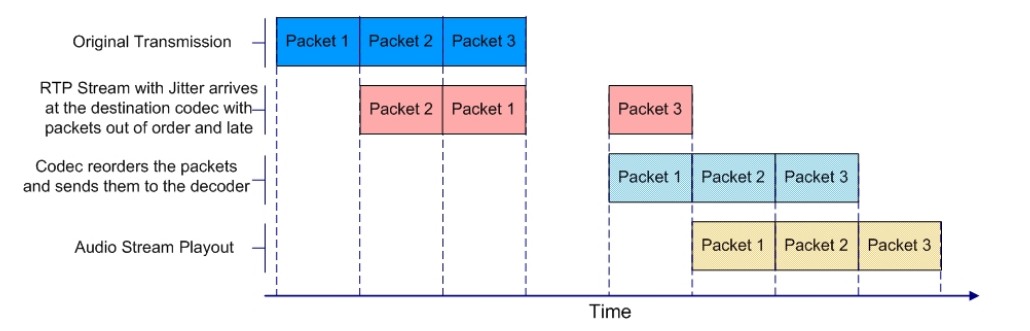
\includegraphics[width=\linewidth]{buf-vis.png}
  		\caption{Visualization of how the buffer works}
  		\label{fig:bufvis}
	\end{figure}
	
	\section{Forward error correction (FEC)}
	\begin{itemize}
		\item Forward error correction (FEC) is an error correction technique to detect and correct a limited number of errors in transmitted data without the need for retransmission.
		\item The sender sends a redundant error-correcting code along with the data frame
		\item The receiver performs necessary checks based upon the additional redundant bits. If it finds that the data is free from errors, it executes error-correcting code that generates the actual frame then removes the redundant bits before passing the message to the upper layers.
		\item Error-correcting code can be broadly categorized into two types, namely, block codes and convolution codes
			\begin{itemize}
				\item \textbf{\emph{Block codes}}: The message is divided into fixed-sized blocks of bits to which redundant bits are added for error correction
				\item \textbf{\emph{Convolutional codes}}: The message comprises of data streams of arbitrary length and parity symbols are generated by the sliding application of a Boolean function to the data stream
			\end{itemize}
	\end{itemize}
	
	\chapter{Chapter 6: Synchronization}
	\newpage
	\section{Give two examples to demonstrate the importance and the need of synchronization mechanism between processes in distributed systems}
\begin{itemize}
	\item Distributed System is a collection of computers connected via the high speed communication network.
	\item The hardware and software components communicate, coordinate their actions and share their resources to other nodes by message passing.
	\item There is need of proper allocation of resources to preserve the state of resources and help coordinate between the several processes.
	\item Example: If a distributed system is not synchronized, for example computer A is 10 minutes behind computer B and both computer is on the same timezone (say ICT) with computer B is synchronized with the standard time in timezone. At 7:00 am Hanoi time, computer A try to write something to the shared resources and register the timestamp as 7:00 Hanoi time, but since it is technically 7:10 am, the system will not let the user from A to write anything because the timestamp is invalid. In fact, users from computer A cannot write anything until the administrator synchronizes that machine. Timestamp invalidation can also caused lagging when using real time application or application that shared the resources to a lot of users like online games or chat applications.
	\item Benefit of synchronization through example: With synchronization, when playing online games for example, since most packages have to have a timestamp or a related time series to determine the player model action sequences, with synchronization, there can be less lag and enable better quality for player. In fact, nowadays, most online games required you to synchronized before playing. 
\end{itemize}

\section{Compare Network Time Protocol and Berkeley algorithm}
\begin{tabular}{|c|c|}
\hline 
Berkeley Algorithm & Network Time Protocol \\ 
\hline 
Having 1 Master to be standard & Having 3 classes with \\ & class 1 is the highest accuracy and\\ & class 3 is the lowest \\ 
\hline 
Master calculate the & Class 1 is the standard. Class 2 get time \\ average time and discard outliers & from Class 1 and Class 2 server. \\ & Class 3 get time from any server \\ & when they attempted connecting to one \\ 
\hline 
Send time adjustment to clients  & Send timestamp to be changed into \\ 
\hline 
Round trip message & One way message to dictate time \\ 
\hline 
\end{tabular}

\section{What is the typical characteristic of synchronization algorithm for wireless networks}
Since the primary concern of all wireless applications is energy conservation, the typical characteristics of synchronization algorithm for wireless networks are :
\begin{itemize}
	\item It must carefully regiment its frequency of resynchronization, and avoid flooding. 
	\item In addition, the algorithm cannot typically rely on a power-hungry source of real time such as GPS. 
	\item Another characteristic of wireless networks is unexpected and possibly frequent changes in network topology. Thus, a CSA in a wireless medium must continue to function in the face of node failures and recoveries. 
	\item Lastly, many applications in wireless settings are local in nature. That is, only nearby nodes in the network need to participate in some activity. Thus, a desirable property for a CSA is that it closely synchronizes nodes which are nearby, while possibly allowing faraway nodes to be more loosely synchronized.
\end{itemize}

\section{What is the difference between physical synchronization and logical synchronization}
\begin{tabular}{|c|c|}
\hline 
Physical Synchronization & Logical Synchronization \\ 
\hline 
Synchronize the exact timestamp & Synchronize by order of action \\ 
\hline 
Must change the clock in each systems & No need to change the clock \\  based on a standard &\\
\hline 
Maintain the same notion of time & Keep track of information pertaining \\ & to the order of events \\ 
\hline 
Expensive to maintain & Inexpensive to maintain \\ 
\hline 
Inherently inaccurate & Fairly inherently accurate \\ 
\hline 
\end{tabular}

\section{What are the update steps of counters to implement Lamport’s logical clock}
\begin{itemize}
	\item Once the logical clock function has an event, it looks at the time on that event, and compares it to the time on the clock’s process
	\item It chooses the larger of the options, and increments it arbitrarily
\end{itemize}

\section{Answer questions based on an algorithm for the physical clock synchronization}
\begin{enumerate}[label=\alph*)]
	\item Is the value of $T_P$ calculated by the above formula absolutely accurate?
	\begin{itemize}
		\item Given that there is a constant delay on the medium, the value $T_P$ can be consider absolutely accurate because $RTT$ is double the one way time in that condition and $T_P$ will be equal with the timer on server S at that time.
		\item In practice, the value $T_P$ is not absolutely accurate but it can be consider as accurate enough to use.
	\end{itemize}
	\item Let $\delta$ be the deviation of time value and $min$ the minimum time value it takes to transmit a message one-way. Determine the value $\delta$ using only 2 variables $RTT$ and $min$
	\begin{itemize}
		\item If there is no deviation of time value, $RTT = 2*min$
		\item The deviation of time value is the different between $RTT$ and two time the $min$. So the equation would be:
		\[\delta = RTT - 2*min\]
		\item $\delta$ should be positive but it can be negative when you upgrade to a better system and/or better medium. When that happened, you need to update your $min$ value. 
	\end{itemize}
\end{enumerate}

\section{Answer the following questions in regard of using the Vector Clock concept for enforcing causal communication}
\begin{enumerate}[label=\alph*)]
	\item List  two  conditions  the receiving process use to check whether the message satisfies causality.
	\[\bigg\{
	\begin{matrix}
		V_{Pj}[i] = V_S[i] - 1\\
		V_{Pj}[k] \geq V_S[k] \forall k \in [1, 2, 3, ..., n] - \{i\}
	\end{matrix}
	\]
	\item Vector clock values for 4 points $X1$, $X2$, $X3$, and $X4$
	\[X1 = (0,1,0)\]
	\[X2 = (1,1,0)\]
	\[X3 = (2,1,1)\]
	\[X4 = (2,1,2)\]
	\item Message will be kept at the middleware level:
	Message b
\end{enumerate}

\section{What is a mutual exclusion algorithm in a distributed system}
\begin{itemize}
	\item Mutual exclusion: Concurrent access of processes to a shared resource or data is executed in mutually exclusive manner.
	\item Only one process is allowed to execute the critical section (CS) at any given time.
	\item In a distributed system, shared variables (semaphores) or a local kernel cannot be used to implement mutual exclusion.
	\item Message passing is the sole means for implementing distributed mutual exclusion.
	\item Distributed mutual exclusion algorithms is the family of algorithms that deals with unpredictable message delays and incomplete knowledge of the system state.
\end{itemize}

\section{What is the drawback of the centralized algorithm for the mutual exclusion}
\begin{itemize}
	\item If the coordinator crashes, the entire system may go down with it since it is a single point of failure.
	\item If processes normally block after making a request, they cannot distinguish a dead coordinator from "permission denied" since no message comes back.
	\item Bottleneck when deploy on the large system with a single coordinator (scalability)
\end{itemize}

\section{What is the drawback of the distributed algorithm for the mutual exclusion}
\begin{itemize}
	\item Algorithm is suitable only for small group of processes.
	\item It is highly complex due to the need of identify all processes needed.
\end{itemize}

\section{Propose a solution for the problem of lost token in Token Ring mutual exclusion algorithm}
When a process (say) P1 wants to enter into its critical
section, it sends request to the coordinator. If the
coordinator retains the token, it then sends the token to the
requesting process (P1). After getting the token, the
process will send an acknowledgment to the coordinator,
and enters the critical section. During the execution of the
critical section, P1 will continually send an EXISTS signal
to the coordinator at certain time interval, so that, the
coordinator becomes acquainted that the token is alive and
it has not lost. As a reply to every EXISTS signal, the
coordinator sends back an OK signal to that particular
process (P1), so that the process that is executing in its
critical section (P1), gets to know that the coordinator is
alive also.\\
Now, suppose, the coordinator is not receiving the
EXISTS signal from that process P1. Here two cases may
appear:
\begin{enumerate}
	\item The coordinator assumes that the token has lost. Then the coordinator will regenerate a new token and sends it to that
process (P1) and again it starts executing its critical
section.
	\item The process P1 may crash or fail while executing in it
critical section and consequently, the coordinator does not
receiving any EXISTS signal from P1. Hence, the coordinator will identify it as a crashed process and update the ring configuration table and send the UPDATE signal with update information to other processes to update their own ring configuration tables.
\end{enumerate}
Again it may be the case, that the process P1 (which is currently executing in its critical section), is not receiving the OK signal form the coordinator. So, P1 would assume that the coordinator is somehow crashed. At this moment, the process P1 will become the new coordinator and complete the critical section execution. The new coordinator will send a message [COORDINATOR (PID)] to every other process, that it becomes the new coordinator and send the UPDATE signal with update information, to update the ring configuration tables maintained by all other
processes.\\
The algorithm also overcomes the overhead of token
circulation in the ring. If no processes in the ring want to
enter in its critical section, then there is no meaning of
circulating the token throughout the ring. Rather, in this
approach, the coordinator will keep the token, until any
other process requests it.
\begin{enumerate}
	\item The algorithm guarantees mutual exclusion, because at
any instance of time only one process can hold the token and can enter into the critical section.
	\item Since a process is permitted to enter one critical
section at a time, starvation cannot occur. 
\end{enumerate}

\section{How many messages does the system need to vote the coordinator}
When P3 starts the election after node P4 and P7 was broken, it will take the system a total of 10 messages to elect a new coordinator.
\begin{itemize}
	\item The first round, P3 sent 4 ELECTION messages to P4, P5, P6 and P7. P3 would receive 2 ANSWER messages from P5, P6.
	\item The second round, P5 sent 2 ELECTION messages to P6 and P7 and received 1 ANSWER message from P6.
	\item The final round, P6 sent 1 ELECTION message to P7 and received 0 ANSWER message thus making it the coordinator.
\end{itemize}

\section{Answer questions with a system the has N nodes and each node has a status table of other nodes and the whole system on election algorithm}
\begin{enumerate}[label=\alph*)]
	\item How many messages do we need to vote the coordinator
	\[number\_of\_messages = 2(N-i-1) + (i+1)N\]
	\item When a broken node become working again
	\begin{itemize}
		\item That broken node first broadcast a WORKING message to each of the other nodes for update their tables. The other working nodes will send a acknowledge message back for that previously broken nodes to update its table.
		\item If the said node has higher id than the current coordinator, the coordinator will sent the ELECTION message to said node, otherwise, the system will continue to run
	\end{itemize}
\end{enumerate}

\section{Answer questions regrading a mutual exclusion algorithm}
\begin{enumerate}[label=\alph*)]
	\item How many messages does the system need to successfully let a process use SR. 
	\begin{itemize}
		\item Suppose there are $k$ REQUEST messages on the queue already $0 \leq k$ (no upper limit due to Pi can post multiple REQUEST messages). Pi will wait $k$ RELEASE messages.
		\item Pi sends $N-1$ REQUEST messages and receives $N-1$ REPLY messages.
		\item The total amount of messages would be:
		\[k + 2(N-1)\]
	\end{itemize}
	\item The improvement will cut all the unnecessary REPLY messages since the purpose of the REPLY was to reorder the priority queues of all processes to timestamp order. The new algorithms can cut at most $N - 1$ REPLY messages. In the worst case scenario, when $ts_i$ is the latest, it will perform like the original algorithms.
\end{enumerate}
\end{document}